% Phụ lục B

\chapter{Sơ đồ chân nối} % Tên của phụ lục

\label{AppendixB} % Để trích dẫn chương này ở chỗ nào đó trong bài, hãy sử dụng lệnh \ref{AppendixB} 

%----------------------------------------------------------------------------------------


\section{Sơ đồ chân nối mô hình điều khiển vị trí góc quay động cơ DC Encoder}

\begin{figure}[h!]
	\centering
	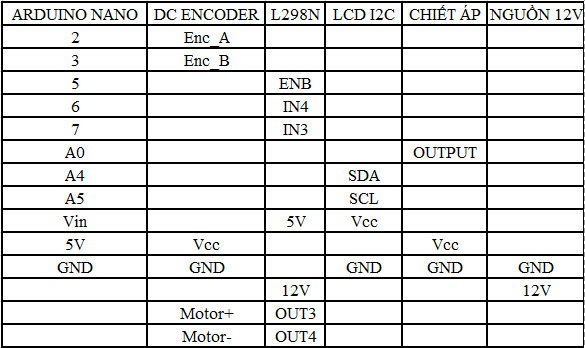
\includegraphics[width=0.8\textwidth]{sd2.png}
	\caption[Sơ đồ chân nối mô hình điều khiển vị trí góc quay động cơ DC Encoder]{Sơ đồ chân nối mô hình điều khiển vị trí góc quay động cơ DC Encoder}
	\label{fig:Sơ đồ chân nối mô hình điều khiển vị trí góc quay động cơ DC Encoder}
\end{figure}



